% EN48 c01 | 原书 p.1–12 及 p.13 上半（§1.2 收尾）（PDF 10–22） | 第 1 章 §1.1–1.2
% 块骨架：标题行已设定，正文由译者填写。每页起首用 % ===== 原书 p.N ===== 注释标记。
% 边界说明：原书第十三页上半仍属 §1.2（三条结果收尾），
% 为保持小节与定理编号连续，归入本块；c02 从 §1.3 起。
\section{引言、背景与设定}

\subsection{论文结果与方法的陈述}

% ===== 原书 p.1 =====
本文中，代词「我们」兼指作者与读者。

\begin{theorem}\label{thm:main}
设 $\iota\colon H := \Sigma_2 \hookrightarrow V$ 为亏格 $2$ 曲线到复维数 $2$ 的阿贝尔簇
$V$ 的嵌入。则存在镜像 $(Y,v_0)$：它是辛纤维丛，纤维记作 $\Vdual$，与 $V$ 互为镜像；
$\Vdual$ 也是复维数 $2$ 的阿贝尔簇。于是有下面的交换图，图中竖直箭头是范畴之间的
上同调意义下全忠实嵌入函子：
\begin{equation}\label{eq:1-1}
\begin{tikzcd}[column sep=4.2em, row sep=3.2em]
\DBCoh(V) \arrow[rr,"i^*"] \arrow[dd, hook, "HMS"'] & & \DBCoh(H) \arrow[dd, hook, "HMS\ (C.)"] \\
& \curvearrowright & \\
H^0(\mathrm{Fuk}(\Vdual)) \arrow[rr,"\sqcup"] & & H^0(\mathrm{FS}(Y,v_0))
\end{tikzcd}
\end{equation}
\end{theorem}

\begin{remark}[图示解释]\label{rem:diagram}
上排是有界相干层导出范畴之间的函子。本例只需考虑线丛。下排是深谷范畴与
Fukaya--Seidel 范畴之间的函子。这些范畴的态射空间是链复形；态射不满足结合律，
但满足涉及任意多个态射的结合关系，所以它们是 $A_\infty$-范畴。本文讨论的是
上同调深谷范畴：对态射群取上同调，得到真正的范畴。用 $A_\infty$-函子构造此图，
即除对象、态射与复合之外还要核对高阶复合映射相符，这是将来的方向。
\end{remark}

\transnote{图中两条竖直箭头的含义不同。左列 $\DBCoh(V)\to H^0(\mathrm{Fuk}(\Vdual))$
的 HMS 仍是猜想，[Fuk02] 只对特定情形证明；右列 $\DBCoh(H)\to
H^0(\mathrm{FS}(Y,v_0))$ 才是本文证明的「HMS (C.)」。两列都只在上同调层面陈述，
因为 $\mathrm{Fuk}$ 与 $\mathrm{FS}$ 本质上是 $A_\infty$-范畴。}

\begin{remark}\label{rem:fuk02}
注意：任意维数与任意商格的阿贝尔簇的 HMS 已在 [Fuk02] 中用更先进的工具讨论过。
本文对这个特例给出另一种论证。
\end{remark}

% ===== 原书 p.2 =====
\begin{remark}[亏格 2 曲线 HMS 的已有工作]\label{rem:seidel}
Seidel 证明了亏格 $2$ 曲面在 A 模型一侧的 HMS [Sei11]，即辛一侧；所以本文考虑
B 模型，即亏格 $2$ 曲线上的复结构。Seidel 构造的复镜像是 $\C^3/\Z_5$ 按旋转群取商的
crepant resolution（保持典范类的解消）：零点处的奇点被解消，同时第一 Chern 类保持不变；
它还配有超势。他论文中超势的临界轨迹与本文的镜像相同。一个未来方向是进一步弄清
他的镜像与本文镜像的关系。注意：我们不在 [Sei08] 的正合情形，即 $\omega$ 不正合——
辛纤维丛的纤维紧致且体积非零；也不在单调情形，后者下文还会讨论。我们处在镜像的
Calabi--Yau 情形：$c_1=0$，且镜像是 Landau--Ginzburg 模型。
\end{remark}

\transnote{$\C^3/\Z_5$ 中的 $\Z_5$ 按旋转作用。crepant resolution 指解消后典范除子
平凡，即 $K_X$ 保持不变，因而 $c_1=0$。这与本文的镜像同为 LG 模型，但 Seidel 的
镜像是代数簇，本文的镜像带有辛形式，二者只在超势的临界轨迹上重合。}

\transnote{「正合」指 $\omega=\de\lambda$ 是恰当形式；「单调」指
$c_1=\lambda[\omega]$（$\lambda>0$）。本文两条都不满足，所以 [Sei08] 的正合
Fukaya 范畴与单调 Fukaya 范畴的技术都不能直接照搬，第 4 章要重新定义
$H^0(\mathrm{FS}(Y,v_0))$。}

\noindent\textit{定理~\ref{thm:main} 的证明纲要。}\ 我们的做法如下：
\begin{itemize}[leftmargin=2.2em,itemsep=0.25em]
\item 把亏格 $2$ 曲线作为超曲面嵌入阿贝尔簇 $V$。
\item 沿 $\Sigma_2\times\{0\}$ 爆破 $V\times\C$，使 $\Sigma_2$ 成为爆破所得 $X$ 上
  某个全纯函数的临界轨迹；这正是 [AAK16] 求环簇中超曲面的 SYZ 镜像所用的办法。
  爆破空间自带一个拉格朗日环面丛。
\item 用 SYZ 得到复镜像 $Y$，它比 $\Sigma_2$ 高两维；再给这个镜像配一个全纯函数
  $v_0$，用它编码与 $\Sigma_2$ 互为镜像的行为。
\item 两侧都是凯勒的，所以改而考虑亏格 $2$ 曲线上的 B 模型，并在镜像上构造 A 模型。
  注意：配对为 Calabi--Yau 时应当有对合性，因此也可以从镜像作 A 模型出发，
  按 [AAK16, §8] 或 [CLL12] 构造 $X$。
\item 对镜像阿贝尔簇，证明上同调层面存在全忠实嵌入。
\item 对 $\Sigma_2$ 与 $(Y,v_0)$ 证明同样的结论。
\item 未来方向：证明所考虑的拉格朗日子范畴生成深谷范畴；把上同调范畴的等价
  加强为 $A_\infty$-等价。
\end{itemize}

\begin{remark}\label{rem:general-type}
我们处在一类一般型情形：亏格 $2$ 曲线上 $c_1<0$，所以镜像是非紧的 LG 模型。
又因为作了爆破，我们处在非环簇的拉格朗日纤维丛的设定中。所谓环簇，指纤维丛来自
矩映射；这里从矩映射出发，然后在底空间上作运算，结果仍是拉格朗日环面丛，
但不再来自矩映射。例如 [AAK16] 中最后一个坐标来自矩映射，其余坐标不是。
$X$ 上的深谷范畴将是 M. Liu 与 J. Hicks 的设定。反过来，
\end{remark}

% ===== 原书 p.3 =====
在 [CLL12] 中，作者取 $Y$ 上的 SYZ 镜像，并处理该情形中出现的球面泡。

\subsection{B 侧流形}

\medskip\noindent\textbf{复几何}\par

\begin{remark}[构造 SYZ 镜像是输入拉格朗日环面丛]\label{rem:sy-input}
给定辛流形上的拉格朗日环面丛，SYZ 构造 [SYZ96] 在同一底空间上指定对偶纤维，
由此得到一个候选的镜像复流形。对偶纤维的点由原纤维上平凡线丛的酉平坦联络参数化。
这一过程在 [Aur07] 中有明确说明。
\end{remark}

构造合适的拉格朗日环面丛是难题。R. Guadagni 的学位论文在环簇退化的中心纤维上
找到了拉格朗日环面丛，这正是本文镜像 $Y$ 的设定。然而 $\Sigma_2$ 上并没有明显的
拉格朗日环面丛，也没有到 $\Sigma_2$ 的环簇退化。Abouzaid--Auroux--Katzarkov
[AAK16] 在环簇中超曲面的爆破上构造了拉格朗日环面丛，本文把它改编到阿贝尔簇的情形。

\begin{definition}[阿贝尔簇的定义]\label{def:abelian-variety}
阿贝尔簇 $V$ 的拓扑型是 $T^4$，复结构定义如下：
\begin{equation}\label{eq:1-2}
\begin{gathered}
V := (\C^*)^2/\Gamma_B\\
\Gamma_B := \Z\langle\gamma',\gamma''\rangle\subset\Z^2,\qquad
\gamma' := \binom{2}{1},\quad \gamma'' := \binom{1}{2}\\
\Gamma_B\curvearrowright(\C^*)^2,\qquad
\gamma\cdot(x_1,x_2) := (\tau^{-\gamma_1}x_1,\tau^{-\gamma_2}x_2)
\end{gathered}
\end{equation}
其中 $\gamma\in\Gamma_B$ 的 $\Z^2$-坐标是 $(\gamma_1,\gamma_2)$，$\tau\in\R$ 参数化
一簇复结构，将来与镜像上一簇辛结构互为镜像。该复结构是通常的 $J_0$ 按 $\Gamma_B$
取商所得；$J_0$ 即在 $(\C^*)^2$ 的每一点上乘以 $i$。
\end{definition}

\begin{remark}[阿贝尔簇的乘法格与加法格视角]\label{rem:additive-mult}
描述阿贝尔簇有等价的方式：格可以像上面那样乘法地作用，也可以像下文那样加法地作用。
后一视角便于理解 $V$ 的上同调，见 [BL04] 与 [Pol03]。

下面的格 $\Gamma$ 加法地作用在 $\C^2$ 上，取商得到乘积环面，记作 $T_B\times T_F$；
它对应上文 $V$ 上乘法复坐标的范数与辐角。我们先定义 $T_B$ 与 $T_F$ 的格，
再定义 $\Gamma$。
\begin{equation}\label{eq:1-3}
\Gamma_B := \Z\Bigl\langle\binom{2}{1},\binom{1}{2}\Bigr\rangle,
\qquad \Gamma_F := \Z^2,
\qquad \Gamma := -\log\tau\cdot\Gamma_B+2\pi i\Gamma_F\subset\C^2
\end{equation}
\end{remark}

\transnote{同一个阿贝尔簇有两种坐标：乘法坐标 $x_i\in\C^*$ 便于描述复结构，
加法坐标 $(u_i,v_i)$ 便于算上同调。二者的桥是
$x_i=\tau^{-u_i}e^{2\pi iv_i}$。下文凡出现 $\Gamma$ 与 $T_B\times T_F$ 都在加法侧，
出现 $(\C^*)^2/\Gamma_B$ 都在乘法侧。}

% ===== 原书 p.4 =====
现在定义带加法结构的阿贝尔簇：
\[
V_+ := \C^2/\Gamma \cong \R^2_{u_1,u_2}/\Gamma_B\times\R^2_{v_1,v_2}/\Gamma_F
=: T_B\times T_F.
\]
加法结构在指数映射下对应乘法结构：
\[
\begin{aligned}
V_+ = \C^2/\Gamma &\ni (-u_1\log\tau+2\pi iv_1,\,-u_2\log\tau+2\pi iv_2)\\
&\xrightarrow{\ \exp\ }
(\tau^{-u_1}e^{2\pi iv_1},\tau^{-u_2}e^{2\pi iv_2})\in V=(\C^*)^2/\Gamma_B.
\end{aligned}
\]
由此可见，$u_1,u_2$ 编码 $V$ 上复坐标 $(x_1,x_2)$ 的范数，$v_1,v_2$ 是辐角。
下标 $B$ 表示矩映射的底空间，矩映射来自标准的 $T^2$-旋转作用
$(\alpha_1,\alpha_2)\cdot(x_1,x_2) := (e^{2\pi i\alpha_1}x_1,e^{2\pi i\alpha_2}x_2)$；
下标 $F$ 表示纤维，即在固定范数 $(|x_1|,|x_2|)$ 下沿轨道旋转角度所得。
特别地，$\Gamma_F$ 在乘法情形不再作用。所以在 $T_F$ 方向，$V_+$ 上的性质应当平凡，
才能经指数映射下降到 $V$。

反方向上，
$\bigl(-\frac{1}{\log\tau}|\log(x)|,\ \frac{1}{2\pi i}(\log(x)-\log|x|)\bigr)$
给出同构 $V\cong T_B\times T_F$，其中 $x=(x_1,x_2)$，这里采用向量记号。
通常 $\tau$ 很小，例如 $\tau=e^{-2\pi}$。当 $\tau\to0$ 时，
$-\log\tau\cdot\Gamma_B$ 中的本原格向量变长。

\begin{claim}[阿贝尔簇 $V$ 的上同调]\label{claim:cohomology}
$H^n(V;\Z)\cong\bigwedge^n\Hom(\Gamma,\Z)$。
\end{claim}

\begin{proof}[{略证，参看 [BL04, §1.3]}]
只需处理 $V_+$，它与 $V$ 同胚。
\[
\Gamma=\pi_1(V_+)=H_1(V_+;\Z)\quad\therefore\quad H^1(V_+;\Z)=\Hom(\Gamma,\Z).
\]
第二个等号因为 $\Gamma$ 交换，且 $H_1$ 是 $\pi_1$ 的交换化。第三个等号由万有系数
定理与无挠得出。于是用 K\"unneth 公式、它与杯积的相容性以及 de Rham 同构，
得到环同构（对 $n$ 归纳）：
\[
\bigwedge^n\Hom(\Gamma,\Z)\cong\bigwedge^n H^1(V;\Z)
\xrightarrow{\ \cup\ }H^n(V;\Z).\qedhere
\]
\end{proof}

\begin{corollary}[{[Pol03, §1]}]\label{cor:line-bundles-top}
$V$ 上复线丛按第一 Chern 类作拓扑分类，第一 Chern 类是反对称双线性形式
$E\colon\Gamma\times\Gamma\to\Z$。
\end{corollary}

\begin{proof}
对复线丛，由前一断言 $c_1(L)\in H^2(V;\Z)\cong\bigwedge^2\Hom(\Gamma,\Z)$，
而 $\bigwedge^2\Hom(\Gamma,\Z)\cong\Hom(\bigwedge^2\Gamma,\Z)$。

我们想知道哪些形式 $E$ 能成为全纯线丛的第一 Chern 类。这恰是那些满足
$c_1(L)\in H^{1,1}(V)$ 的 $L$。所以下一步是考虑 $\mathrm{Pic}(V)$ 与阿贝尔簇上的
Hodge 分解，再像上文拓扑上同调那样用格 $\Gamma$ 给出描述。
\end{proof}

% ===== 原书 p.5 =====
\begin{claim}\label{claim:holomorphic-line-bundles}
$V$ 上全纯线丛由
\begin{equation}\label{eq:1-4}
H^1\bigl(\pi_1(V_+);H^0(\OO^*_{\tilde V_+})\bigr)\cong H^1(V_+,\OO^*)
\end{equation}
分类。
\end{claim}

\begin{proof}[{据 [BL04] 的略证}]
该理论来自 [BL04, 附录 B]，其中式~\eqref{eq:1-4} 左端的元素称为\textbf{自守因子}
（factor of automorphy）。这个同构是复流形上 Cartier 除子与线丛等价性的类比，
只是多了 $\Gamma$-等变性。换言之，自守因子是这样一个函数：其零点集（即除子）
在 $\Gamma$ 作用下不变。群作用的概念等价于上链的概念，所以这种不变性编码在
上同调群 $H^1(\pi_1(V_+);H^0(\OO^*_{\tilde V_+}))$ 中。右端
$H^1(V_+,\OO^*)\cong\mathrm{Pic}(V_+)$ 由 $\C^2/\Gamma$ 上的全纯线丛组成。
注意 $\tilde V_+=\C^2$。

设 $\pi\colon\C^2\to V_+$ 是万有覆盖。式~\eqref{eq:1-4} 的同构构造如下，
参看 [BL04, Proposition B.1]。$V_+$ 上的线丛有很好的描述：$V_+$ 上卡片的
上链条件，等价于 $\Gamma$ 在万有覆盖中一族卡片上作用；这些卡片是底空间开集的
提升。下面来说明。
\begin{itemize}[leftmargin=2.2em,itemsep=0.25em]
\item 设 $\{U_i\}$ 是 $V_+$ 的覆盖。全纯线丛由过渡函数 $g_{ij}$ 把 $U_i\times\C$
  粘到 $U_j\times\C$ 定义；$g_{ij}$ 全纯，作用在 $\C$ 因子上。等价地，可以把每个
  $U_i$ 提升为 $W_i$，使 $\pi|_{W_i}\colon W_i\to U_i$ 是双全纯。特别地，
  $\pi_i^{-1}(x)$ 与 $\pi_j^{-1}(x)$ 是同一点的两个提升；由万有覆盖的定义，
  它们相差某个 $\gamma_{ij}\in\Gamma$。
\item 于是可以把过渡函数看成两个变量的函数：一个提升，以及记录
  $\pi_i^{-1}(x)$ 到 $\pi_j^{-1}(x)$ 变化的 $\gamma_{ij}$。即
  $\pi_j^{-1}(x)=\gamma_{ij}\pi_i^{-1}(x)$，其中 $\gamma_{ij}\in\Gamma$。然后定义
  \[
  f\bigl(\gamma_{ij},\pi_i^{-1}(x)\bigr) := g_{ij}.
  \]
\item 因为 $\Gamma$ 作用在 $\C^2$ 上，群作用给出 $\gamma_{ij}\gamma_{jk}=\gamma_{ik}$。
  $g_{ij}$ 是线丛上的上链，这一事实给出
  \begin{equation}\label{eq:1-5}
  \begin{aligned}
  g_{ij}g_{jk} &= g_{ik}\\
  \therefore\quad f\bigl(\gamma_{ij},\pi_i^{-1}(x)\bigr)
    f\bigl(\gamma_{jk},\pi_j^{-1}(x)\bigr)
    &= f\bigl(\gamma_{ik},\pi_i^{-1}(x)\bigr)\\
  \therefore\quad f\bigl(\gamma_{ij},\pi_i^{-1}(x)\bigr)
    f\bigl(\gamma_{jk},\gamma_{ij}\pi_i^{-1}(x)\bigr)
    &= f\bigl(\gamma_{ij}\gamma_{jk},\pi_i^{-1}(x)\bigr)\\
  \Longleftrightarrow\quad [f] &\in H^1\bigl(\Gamma,H^0(\OO^*_{\C^2})\bigr)
  \end{aligned}
  \end{equation}
  也就是说，$f$ 是自守因子。
\item 具体地，考察上链与上边界在映射
  $g_{ij}\mapsto f(\gamma_{ij},\pi_i^{-1}(\cdot))$ 下的像，
  得到 $\Gamma$ 上离散拓扑、取值于层 $\OO^*_{\C^2}$ 的 \v{C}ech 上同调群。
  特别地，像给出 $H^1(\pi_1(V_+);H^0(\OO^*_{\tilde V_+}))$ 中一个类的代表。
\end{itemize}
\end{proof}

\transnote{「自守因子」不是数，而是群 $\Gamma$ 上的函数。它与过渡函数 $g_{ij}$ 的关系
是 $g_{ij}=f(\gamma_{ij},\pi_i^{-1}(x))$：过渡函数记住两点的差 $\gamma_{ij}$，
自守因子把这一差异记录成 $\Gamma$ 上的函数。此处沿用复几何的通行译名，
不译作「自同构因子」。}

% ===== 原书 p.6 =====
\begin{itemize}[leftmargin=2.2em,itemsep=0.25em]
\item 平凡线丛的过渡函数形如 $g_{ij}=h_j/h_i$。于是令
  $g_{ij}=f(\gamma_{ij},\pi_i^{-1})=h_j/h_i$，可在万有覆盖上定义函数 $h$：
  \[
  h\bigl(\pi_i^{-1}(x)\bigr) := h\bigl(\pi_j^{-1}(x)\bigr)\cdot\frac{h_i}{h_j}.
  \]
\item 所以这对应上边界 $(\gamma,\tilde x)\mapsto h(\gamma\cdot\tilde x)h(\tilde x)^{-1}$，
  其中 $h\in H^0(\OO^*_{\C^2})$。
\item 这个对应在上同调上是同构，见 [BL04, Proposition B.1]。
\item 注意对所有更高次上同调也有类似结果。
\end{itemize}

\begin{claim}\label{claim:hodge-11}
$H^{1,1}(V_+)\cong\Hom_{\C}(\C^2,\C)\otimes\Hom_{\bar\C}(\C^2,\C)$。
\end{claim}

\begin{proof}
在复向量空间 $\C^2$ 上有分解 $(\C^2)^{1,0}\oplus(\C^2)^{0,1}$
[Huy05, Lemma 1.2.5]。而 $(T^{1,0}\C^2)^*=\Hom_{\C}(\C^2,\C)$，
$(T^{0,1}\C^2)^*=\Hom_{\bar\C}(\C^2,\C)$，见 [BL04, Theorem 1.4.1]。
设 $t_v$ 是环面上的平移，可以用 $dt_{-v}$ 拉回把 $\C^2$ 上的 $(p,q)$-形式延拓到
整个环面。所以
$H^{1,1}(V_+)\cong\Hom_{\C}(\C^2,\C)\otimes\Hom_{\bar\C}(\C^2,\C)$。\qedhere
\end{proof}

\begin{corollary}[{参看 [BL04, Proposition 2.1.6]}]\label{cor:holomorphic-structure}
复线丛 $\LL$ 有全纯结构，当且仅当 $c_1(\LL)$ 是 $(1,1)$-形式，即
$E(i\cdot,i\cdot)=E(\cdot,\cdot)$，且 $E(\Gamma,\Gamma)\subseteq\Z$。
特别地，$V_+$ 上的全纯线丛对应 $2\times2$ Hermite 矩阵，并满足同样的整性条件。
\end{corollary}

\begin{remark}\label{rem:exponential-sequence}
层的指数短正合列 $0\to\Z\to\OO\xrightarrow{\exp}\OO^*\to1$ 给出长正合列，其中含
\[
H^1(V,\OO^*)\cong\mathrm{Pic}(V)\xrightarrow{\ -c_1\ }H^2(V;\Z)\subseteq H^2(V;\C)
=H^{0,2}(V)\oplus H^{1,1}(V)\oplus H^{2,0}(V).
\]
特别地，$c_1(\LL)\in H^{1,1}(V)$，当且仅当它与 $H^{0,2}$、$H^{2,0}$ 的生成元作楔积
得零。

注意 $H(\cdot,\cdot) := E(i(\cdot),\cdot)+iE(\cdot,\cdot)$ 是 Hermite 形式，
见 [Huy05, Lemma 1.2.15]。用乘子 $e_\gamma$（[BL04] 中称自守因子）定义 $\LL$，
即 $\Gamma\to\OO^*(V)$；它描述绕 $\pi_1(V)$ 中元素一圈时线的、必然 $\Gamma$-周期的
粘合函数。
\end{remark}

\transnote{约定 $E=\mathrm{Im}\,H$，$H$ 是 Hermite 形式（对第二变量共轭线性）。
$E(i\cdot,i\cdot)=E(\cdot,\cdot)$ 等价于 $E$ 是 $(1,1)$-型；这一步把拓扑分类与
全纯分类接起来。下文推论~\ref{cor:symmetric-matrix} 用它把 $E$ 化成实对称矩阵。}

\begin{lemma}[{参看 [Pol03, Theorem 1.3] 与 [BL04, Appell--Humbert Theorem 2.2.3]}]\label{lem:picard}
$V_+$ 上全纯线丛的 Picard 群 $\mathrm{Pic}(V_+)$ 同构于所有满足下述条件的对
$(H,\alpha)$ 的集合：$H\colon\C^2\times\C^2\to\C$ 是 Hermite 形式，
$\mathrm{Im}\,H(\Gamma,\Gamma)\subseteq\Z$，$\alpha\colon\Gamma\to U(1)$，且
\[
\alpha(\gamma+\tilde\gamma)=\exp\bigl(\pi iE(\gamma,\tilde\gamma)\bigr)
\alpha(\gamma)\alpha(\tilde\gamma),
\]
其中 $E=\mathrm{Im}\,H$。
\end{lemma}

\begin{proof}[{据 [Pol03, 第 2 章] 与 [BL04, 第 2 章] 的略证}]
在 [Pol03, §2.3] 中，Polishchuk 说明全纯结构由满足
$\alpha(\gamma+\tilde\gamma)=\exp(\pi iE(\gamma,\tilde\gamma))\alpha(\gamma)
\alpha(\tilde\gamma)$ 的 $\alpha\colon\Gamma\to U(1)$ 参数化；
[BL04, Proposition 2.2.2] 同此（前者的 $\alpha$ 在后者中记作 $\chi$）。
于是选定 $(H,\alpha)$（其中 $E=\mathrm{Im}\,H$）后，自守因子为
\[
(\gamma,v)\mapsto\alpha(\gamma)
\exp\Bigl(\pi H(v,\gamma)+\frac{\pi}{2}H(\gamma,\gamma)\Bigr).
\]
\end{proof}

% ===== 原书 p.7 =====
从 [BD16] 的角度看，这个自守因子是自然的定义；那里有广义 Heisenberg 群的概念。
本文的相关群是半直积 $U(1)\times\C^2$，群律为
\[
(\gamma,v)\cdot(\tilde\gamma,\tilde v)
=\bigl(\exp(\pi iE(v,\tilde v))\gamma\tilde\gamma,\ v+\tilde v\bigr).
\]
Heisenberg 群的关键点在于酉不可约表示的唯一性，这是 Stone--von Neumann 定理。
Fock 表示给出上面的自守因子。

反过来，设全纯线丛 $\LL$ 有自守因子 $f$。由于 $f$ 处处非零，可写
$f=\exp(2\pi ig)$，其中 $g$ 全纯。于是由 [BL04, Theorem 2.1.2]，第一 Chern 类对应
交错形式
\[
E_{\LL}(\gamma,\tilde\gamma)
=g(\tilde\gamma,v+\gamma)+g(\gamma,v)-g(\gamma,v+\tilde\gamma)-g(\tilde\gamma,v),
\]
对任意 $\gamma,\tilde\gamma\in\Gamma=-\log\tau\,\Gamma_B+2\pi i\Gamma_F$ 与任意
$v\in\C^2$ 成立（该式其实与 $v$ 无关）。如上所见，$\LL$ 全纯时 $E$ 对应 Hermite
形式，且 $E(\Gamma,\Gamma)\subseteq\Z$。还可如 [BL04, 第 31 页] 末尾所述构造
$\alpha\colon\Gamma\to U(1)$。这就完成了引理中同构的略证。

\begin{example}\label{ex:alternating-form}
回忆阿贝尔簇上复线丛的 $c_1(L)$ 可由交错形式 $E\colon\Gamma\times\Gamma\to\Z$
（$\Gamma\subset\C^2$）表示。于是取 $\R$-线性组合，可把它延拓为 $\R$-线性形式
$E\colon\C^2\times\C^2\to\R$。关于注~\ref{rem:additive-mult} 中 $\Gamma_B$ 与
$\Gamma_F$ 的生成元所给的基，这给出一个 $4\times4$ 反对称矩阵，按
$\Gamma_B\times\Gamma_F$ 分块。

在本文的设定中，我们希望线丛在 $T_F$ 方向平凡。即对 $v,w\in\Z^2$ 有
$E(iv,iw)=0$。$\LL$ 全纯时，由推论~\ref{cor:holomorphic-structure} 可知
$E(iv,iw)=E(v,w)$。于是 $E$ 是分块矩阵
\[
E=\begin{array}{c|cc}
 & \Gamma_B & \Gamma_F\\\hline
\Gamma_B & 0 & *\\
\Gamma_F & -* & 0
\end{array}
\]
\end{example}

\transnote{原文此处作 ``Remark 1.3''，按上下文应指上面的注~\ref{rem:additive-mult}，
疑为笔误。译文按注~\ref{rem:additive-mult} 处理，并在报告中登记。}

% ===== 原书 p.8 =====
由此得到推论~\ref{cor:holomorphic-structure} 的一个推论。

\begin{corollary}\label{cor:symmetric-matrix}
经 $\exp$ 下降到 $V$ 上全纯线丛的 $V_+$ 上全纯线丛，对应实整对称 $2\times2$ 矩阵。
\end{corollary}

\begin{proof}
在 $V_+$ 上，取 $\Gamma_B+i\Gamma_F$ 的一般元素代入 $E(\gamma+iw,\tilde\gamma+iv)$。
由上文，它是某个 Hermite 形式 $H$ 的 $\mathrm{Im}\,H$；对
$H=\begin{pmatrix}a&b\\ \bar b&a\end{pmatrix}$ 有 $a\in\R$。
\begin{equation}\label{eq:1-6}
(\gamma_1+iw_1\ \ \gamma_2+iw_2)
\begin{pmatrix} a & b+ic\\ b-ic & d\end{pmatrix}
\binom{\tilde\gamma_1+iv_1}{\tilde\gamma_2+iv_2}
\end{equation}
特别地，由 $E(iw,iv)=0$ 得
\begin{align*}
E(iw,iv) &= \mathrm{Im}\,H(iw,iv)
 = \mathrm{Im}\bigl(aw_1v_1+bw_1v_2+icw_1v_2+bw_2v_1+dw_2v_2-icv_1w_2\bigr)\\
 &= c(w_1v_2-v_1w_2)=0\qquad\forall w,v\in\Z^2\\
\therefore\quad c &= 0,
\end{align*}
且 $H$ 实，因而对称。\qedhere
\end{proof}

\transnote{原文先写 $H=\begin{pmatrix}a&b\\ \bar b&a\end{pmatrix}$（对角元相同），
式~\eqref{eq:1-6} 却用一般 Hermite 矩阵
$\begin{pmatrix}a&b+ic\\ b-ic&d\end{pmatrix}$。下文由 $c=0$ 推出 $H$ 实对称，
回到前一种形式；读时把前者看作最终形式的预告即可。此处记号不统一，保留原样，
报告已登记。}

\begin{corollary}\label{cor:factor-form}
$V$ 上全纯线丛可用自守因子
\[
(\gamma,x)\mapsto x^{\lambda(\gamma)}\tau^{\kappa(\gamma)}
\]
表达；其中 $\lambda\in\operatorname{hom}(\Gamma_B,\Z^2)
=\operatorname{hom}(\Gamma_B,\Gamma_F^*)$ 对应第一 Chern
类，$\kappa(\gamma)$ 是实二次多项式：其二次部分由第一 Chern 类决定，
其线性部分决定全纯结构。
\end{corollary}

\begin{proof}
上文所述的自守因子（或见 [Pol03, Equation (1.2.2)] 及其后的讨论）对应某个
$(H,\alpha)$ 的选取，等于
\[
(\gamma,v)\mapsto\alpha(\gamma)\exp\Bigl(\pi H(v,\gamma)+\frac{\pi}{2}H(\gamma,\gamma)\Bigr).
\]
我们计算指数中的表达式（注意本情形中 $\Gamma$ 的元素是
$\gamma+iw\in\Gamma_B+i\Gamma_F$）：
\begin{align*}
&\pi H\Bigl(-\frac{1}{\log\tau}\log x,\ \gamma+iw\Bigr)
 +\frac{\pi}{2}H(\gamma+iw,\gamma+iw)\\
&\quad=\pi\Bigl[-\frac{1}{\log\tau}(\log x)^TH\gamma
 +\frac{1}{2}H(\gamma,\gamma)+\frac{1}{2}H(w,w)\Bigr]
 +i\pi\Bigl(-\frac{1}{\log\tau}\Bigr)\bigl[(\log x)^THw\bigr]\\
&\quad=\pi\Bigl[\Bigl(-\frac{1}{\log\tau}\Bigr)(\log x)^TH\gamma
 +\frac{1}{2}H(\gamma,\gamma)\Bigr]
\end{align*}
\end{proof}

% ===== 原书 p.9 =====
第二行用到 $H$ 实且对称；第三行取 $w=0$，因为结果不应依赖 $\Gamma_F$ 方向的辐角。
于是可令
\begin{align}
(-\log\tau)\lambda(\gamma) &:= H\gamma \notag\\
\kappa(\gamma) &:= \frac{1}{2}H(\gamma,\gamma)+\log(\alpha(\gamma))
\label{eq:1-7}
\end{align}
其中 $H(\Gamma_B,\Gamma_B)\subseteq(-\log\tau)\Z$。本文所用的 $H$ 由下面的例子给出。

\begin{example}\label{ex:H-choice}
回忆例~\ref{ex:alternating-form}。令
\[
H := (-\log\tau)\begin{pmatrix}2&1\\1&2\end{pmatrix}^{-1}.
\]
于是这定义了
\begin{align*}
&\LL\to V\\
&\LL=(\C^*)^2\times\C/\Gamma_B,\qquad
\gamma\cdot(x_1,x_2,v) := (\tau^{-\gamma_1}x_1,\tau^{-\gamma_2}x_2,
\tau^{\kappa(\gamma)}x^{\lambda(\gamma)}v)\\
&\Hom(\Gamma_B,\Z^2)\ni\lambda\colon
\gamma'\mapsto\binom{1}{0},\quad \gamma''\mapsto\binom{0}{1}\\
&\kappa(n_1\gamma'+n_2\gamma'') := -\frac{1}{2}
(n_1\ \ n_2)\begin{pmatrix}2&1\\1&2\end{pmatrix}\binom{n_1}{n_2}
\end{align*}
\end{example}

\begin{claim}\label{claim:kappa-cocycle}
$\kappa(n_1\gamma'+n_2\gamma'')=-\frac{1}{2}n^T
\begin{pmatrix}2&1\\1&2\end{pmatrix}n$ 满足上链条件。
\end{claim}

\begin{proof}
我们要求上述 $\kappa$ 的定义满足群作用的要求
$\gamma^2\cdot(\gamma^1\cdot(x,v))=(\gamma^2\circ\gamma^1)\cdot(x,v)$。
\begin{align*}
(x_1,x_2,v)&\xrightarrow{\gamma^1}
\bigl(\tau^{-\gamma^1_1}x_1,\tau^{-\gamma^1_2}x_2,
\tau^{\kappa(\gamma^1)}x^{\lambda(\gamma^1)}v\bigr)\\
(x_{new},v_{new}) &:= \bigl(\tau^{-\gamma^1_1}x_1,\tau^{-\gamma^1_2}x_2,
\tau^{\kappa(\gamma^1)}x^{\lambda(\gamma^1)}v\bigr)\\
&\xrightarrow{\gamma^2}
\bigl(\tau^{-\gamma^2_1-\gamma^1_1}x_1,\tau^{-\gamma^2_2-\gamma^1_2}x_2,
\tau^{\kappa(\gamma^2)}x_{new}^{\lambda(\gamma^2)}v_{new}\bigr)\\
&=\bigl(\tau^{-\gamma^2_1-\gamma^1_1}x_1,\tau^{-\gamma^2_2-\gamma^1_2}x_2,
\tau^{\kappa(\gamma^2)}(\tau^{-\gamma^1}x)^{\lambda(\gamma^2)}
(\tau^{\kappa(\gamma^1)}x^{\lambda(\gamma^1)}v)\bigr)\\
&=\bigl(\tau^{-\gamma^1-\gamma^2}x,\ 
\tau^{\kappa(\gamma^1)+\kappa(\gamma^2)-\langle\gamma^1,\lambda(\gamma^2)\rangle}
x^{\lambda(\gamma^1)+\lambda(\gamma^2)}v\bigr).
\end{align*}
另一方面，作用 $\gamma^2\circ\gamma^1$ 得
\[
(x_1,x_2,v)\mapsto
\bigl(\tau^{-\gamma^1-\gamma^2}x,\
\tau^{\kappa(\gamma^1+\gamma^2)}x^{\lambda(\gamma^1+\gamma^2)}v\bigr).
\]
\end{proof}

% ===== 原书 p.10 =====
已知 $\lambda$ 是同态。所以要核对两个映射一致，只需核对
\[
\kappa(\gamma^1)+\kappa(\gamma^2)-\langle\gamma^1,\lambda(\gamma^2)\rangle
=\kappa(\gamma^1+\gamma^2).
\]
二次型满足此式，所以我们选形式 $M:=\begin{pmatrix}2&1\\1&2\end{pmatrix}$，
使后文图形的几何处于标准形式。定义
\[
\kappa(n_1\gamma'+n_2\gamma'')=-\frac{1}{2}n^T
\begin{pmatrix}2&1\\1&2\end{pmatrix}n.
\]
则两端都等于
$-\frac{1}{2}n^1Mn^1-\frac{1}{2}n^2Mn^2-n^1Mn^2$，因为按定义 $\gamma^1=Mn^1$、
$\lambda(\gamma^2)=n^2$。

\transnote{$\kappa$ 取二次型不是任意的：上链条件
$\kappa(\gamma^1)+\kappa(\gamma^2)-\langle\gamma^1,\lambda(\gamma^2)\rangle
=\kappa(\gamma^1+\gamma^2)$ 正是二次型与双线性型的极化恒等式。
选 $M=\begin{pmatrix}2&1\\1&2\end{pmatrix}$ 只为让后文图形
（图~\ref{fig:1-1} 及 §1.3 的矩多面体）落在标准位置。}

\begin{claim}\label{claim:sections-periodic}
$V$ 上线丛的截面是 $(\C^*)^2$ 上的函数，满足周期性
\[
s(\gamma\cdot x)=\tau^{\kappa(\gamma)}x^{\lambda(\gamma)}s(x),
\]
因此有 Fourier 展开。
\end{claim}

\begin{proof}
截面 $s\colon V\to\LL$ 必须与线丛有相同的过渡函数（若考虑 Cartier 数据）：
\[
s(\gamma\cdot x)/s(x)=\tau^{\kappa(\gamma)}x^{\lambda(\gamma)}.\qedhere
\]
\end{proof}

\begin{corollary}\label{cor:basis-sections}
设 $\LL$ 是上文定义的次数 $(1,1)$ 线丛。则 $H^0(V,\LL^{\otimes l})$ 有以下截面基：
\[
s_{e,l} := \sum_{\gamma}\tau^{-l\kappa(\gamma+\frac{\gamma_{e,l}}{l})}
x^{-l\lambda(\gamma)-\lambda(\gamma_{e,l})},
\]
其中 $\gamma_{e,l}=s\gamma'+t\gamma''$，$0\le s,t<l$。
\end{corollary}

\begin{claim}[亏格 2 曲线]\label{claim:genus2-hypersurface}
$H=\Sigma_2$ 是 $V$ 中由截面 $s\colon V\to\LL$ 的零点定义的超曲面：
\begin{equation}\label{eq:1-8}
s(x)=\sum_{\gamma\in\Gamma_B}x^{-\lambda(\gamma)}\tau^{-\kappa(\gamma)}.
\end{equation}
\end{claim}

\begin{proof}
由伴随公式，$T^*H=K_H\cong(K_V\otimes\LL)|_H$。因为 $V$ 是阿贝尔簇，
其切丛平凡化，所以 $K_H\cong\LL|_H$。回忆
$\deg(K_H)=\int_H c_1(K_H)=\int_H c_1(\LL)=2g-2$。由于 $\LL$ 在 $x_1$ 与 $x_2$
方向各绕一次得到，其次数为 $2$，故 $g=2$。另一方面，见图~\ref{fig:1-1}：
蓝实线表示 $s(x)$ 零点的行为，那里 $|x_i| =: \tau^{-\xi_i}$ 很大，
等价于 $\tau\approx0$，其中变量 $\xi_i$ 定义为 $-\log_\tau|x_i|$。
\end{proof}

\transnote{$\deg(K_H)=2g-2$ 对亏格 $g$ 的曲线成立。这里 $\LL|_H\cong K_H$ 且
$\deg\LL=2$，所以 $2g-2=2$，得 $g=2$。注意「$\LL$ 绕一次」指在 $x_1$、$x_2$
两个方向上各绕基本域一周。}

% ===== 原书 p.11 =====
当 $\tau\to0$ 时，$s$ 零点的极限用虚线表示。于是把基本域平行四边形的对边粘合、
再旋转 $2\pi$，便得到亏格 $2$ 曲线。下文用函数的热带化概念更详细地描述这一极限行为。

\begin{figure}[htbp]
\centering
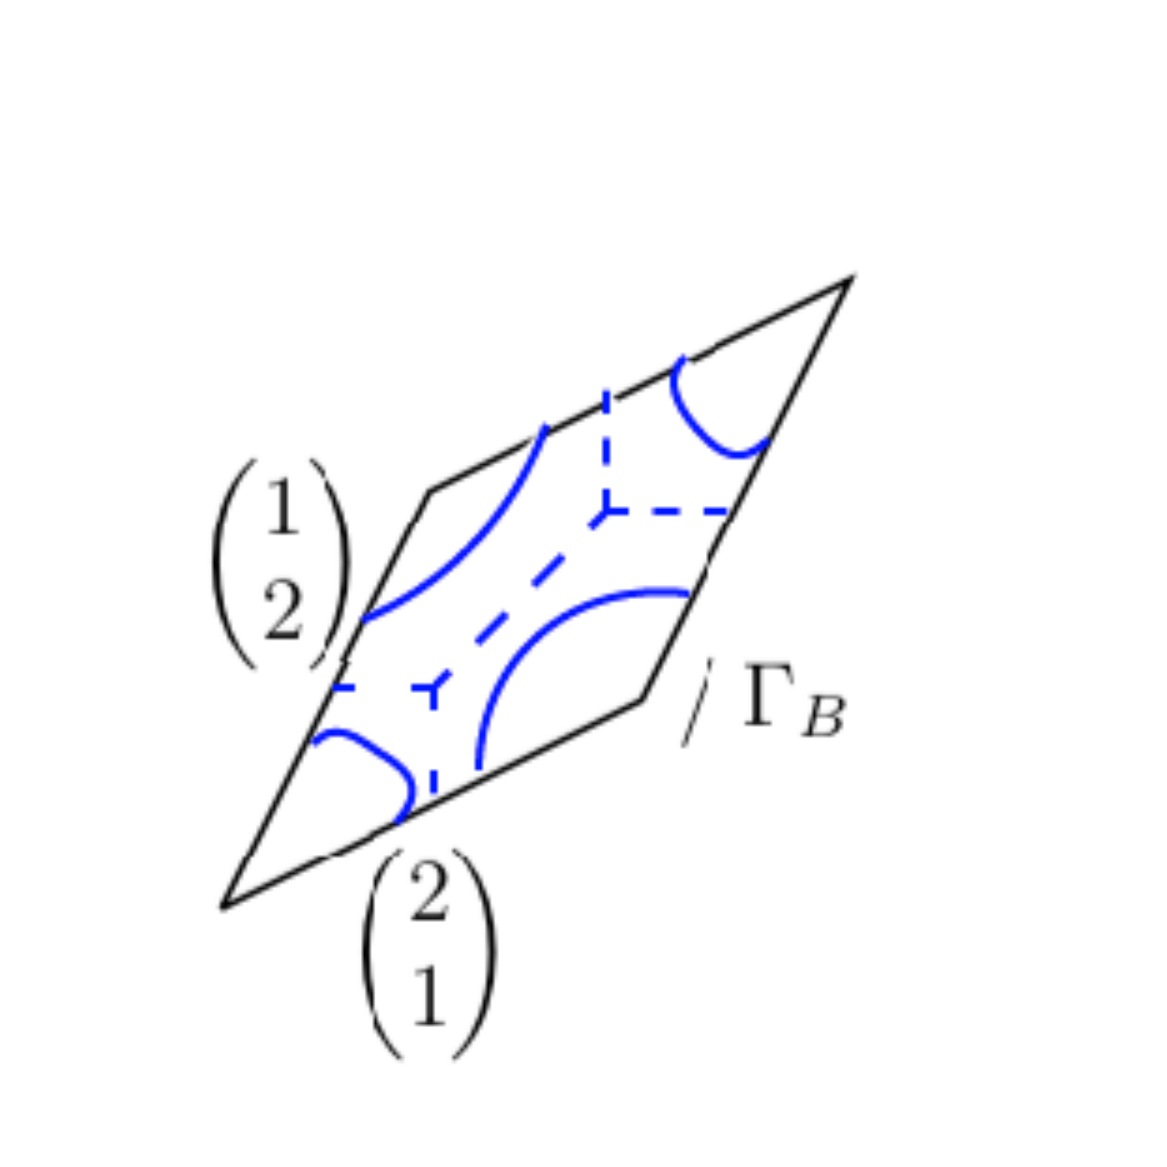
\includegraphics[width=0.42\textwidth]{figures/fig_1_1.png}
\caption{按 $\Gamma_B$ 取商（原书 p.11）}\label{fig:1-1}
\end{figure}

\transnote{图中蓝实线是 $\tau$ 很小时 $s(x)=0$ 的位置，四条蓝弧在粘合对边后两两
相接；虚线是 $\tau\to0$ 的极限（热带曲线），即后文热带化讨论的雏形。
「旋转 $2\pi$」指把平行四边形的斜边方向转正。图内标注 $/\,\Gamma_B$ 与两个
列向量保留原样，不译。}

\begin{remark}\label{rem:lattice-choice}
上文选取的 $\Gamma_B$ 格产生图~\ref{fig:1-1} 中由水平与垂直线段组成的蓝曲线，
本文通篇使用它。换一组生成元会得到不同的图，但本文的方法应当相同。
\end{remark}

\medskip\noindent\textbf{$X$ 与 $H$ 上不变量的关系}\par

\begin{theorem}[{拉格朗日环面丛的构造，取自 [AAK16, §4]}]\label{thm:lagrangian-fibration}
回忆 $x=(x_1,x_2)$ 是 $V$ 上的周期坐标。设 $y\in\C$ 是 $\C$ 因子上的坐标，
$s\colon V\to\LL$ 是上文定义的函数。然后定义
\begin{equation}\label{eq:1-9}
\begin{aligned}
X &:= \mathrm{Bl}_{H\times\{0\}}V\times\C\subset\PP(\LL\oplus\OO)\\
  &= \operatorname{graph}[s(x):y]\\
  &= \bigl\{(x,y,[s(x):y])\in(\PP(\LL\oplus\OO)\to V\times\C)\bigr\}\\
  &= \bigl\{(x,y,[u:v])\mid s(x)v=yu\bigr\},
\end{aligned}
\end{equation}
它是 $V\times\C$ 上 $\PP^1$-丛 $\PP(\LL\oplus\OO)$ 的子集。断言是：$X$ 带有
拉格朗日环面丛。
\end{theorem}

\begin{proof}[证明想法]
环簇有自然的环面作用（其一条轨道在簇中稠密），这个环面作用经矩映射自然给出
拉格朗日环面丛。$y$ 坐标上还有 $S^1$ 旋转作用。在矩映射的底空间上作剪切与粘贴，
对应总空间的爆破，由此在 $X$ 上得到拉格朗日环面丛。\qedhere
\end{proof}

% ===== 原书 p.12 =====
\begin{lemma}\label{lem:critical-locus}
$H=\mathrm{Crit}(y)$。
\end{lemma}

\begin{proof}
零纤维是 $V$ 的真变换与例外除子的并。设 $p$ 是收缩映射（blow-down map）：
\[
p\colon X\to V\times\C,\qquad (x,y,(u:v))\mapsto(x,y).
\]
真变换（proper transform）的定义是
\[
\tilde V := \overline{p^{-1}(V\setminus H\times\{0\})}.
\]
几何上 $\tilde V$ 是 $V$ 的一份拷贝，即爆破中 $V$ 远离 $H$ 那部分的闭包，
它补全了 $V$ 拷贝的其余部分。再定义由收缩映射在 $H$ 上给出的 $\PP^1$-丛，
以及该丛的一个截面 $s^p$：
\begin{align*}
\text{例外除子 } E &:= \{(x,0,(u:v))\mid x\in H\}=p^{-1}(H\times\{0\})\\
p|_E &\colon E\to H\times\{0\}\\
s^p &\colon H\to E,\qquad s^p(x) := (x,0,(1:0)).
\end{align*}
现在可把 $H$ 看成 $y$ 纤维丛的临界轨迹，即旋转 $y$ 的 $S^1$-作用的不动点集，
该作用为 $(x,e^{i\theta}y,(e^{-i\theta}u:v))$。
\begin{align*}
y^{-1}(0) &= \{(x,0,(u:v))\mid s(x)v=0\cdot u\}\\
&= \{(x,0,(1:0))\}\cup\{(x,0,(u:v))\mid s(x)=0\}\\
&= \tilde V\cup E.
\end{align*}
断言是 $\tilde V$ 与 $E$ 交于 $s^p(H)\cong H$。属于 $E$ 意味着 $s(x)=0$，
故 $x\in H$。属于 $\tilde V$ 意味着 $v=0$，故可把 $u\neq0$ 伸缩为 $u=1$。因此
\[
\tilde V\cap E=s^p(H)\cong H=\mathrm{Crit}(y).\qedhere
\]
\end{proof}

\medskip\noindent\textbf{辛不变量}\par

\begin{remark}\label{rem:dim1}
若 $\dim_{\C}V=1$，则 $y\colon X\to\C$ 的零纤维涉及形如 $ab=0$ 的正规交叉除子，
由维数原因产生一个 Lefschetz 奇点。于是可用 Seidel 的 Lefschetz 纤维丛的深谷范畴
[Sei08]；此时 $H$ 是一个点。我们想要该深谷范畴的类比，以 $H=\Sigma_2$ 为临界轨迹，
这需要升高一维。
\end{remark}

\begin{proposition}[{提出 Morse--Bott 纤维丛的深谷范畴 [AAK16]}]\label{prop:morse-bott}
$H\times0$ 在 $V\times\C$ 中的法丛是 $\LL\oplus\OO$。沿 $H\times\{0\}$ 爆破后，
$H=\Sigma_2$ 是正规交叉奇点中两个除子的交，并构成 Morse--Bott 纤维丛
$y\colon(x,y,(u:v))\mapsto y$ 的临界轨迹。于是 [AAK16, Corollary 7.8] 猜想
$\mathrm{Fuk}(H)$ 等价于 AAK 所描述的深谷范畴 $F_s(X,y)$，
因为 $H$ 中的拉格朗日可以从中纤维平行移动，得到 $X$ 中关于超势 $y$ 可容的
非紧拉格朗日。
\end{proposition}

\transnote{Lefschetz 纤维丛的临界点是孤立的；Morse--Bott 纤维丛的临界轨迹 $H$ 是
正维数的子流形，法丛的负特征值方向沿 $H$ 整体存在。这正是本文能用
$H=\Sigma_2$ 作临界轨迹、并把 $H$ 中的拉格朗日平行移动到 $X$ 中的原因。}

% ===== 原书 p.13 =====
\medskip\noindent\textbf{复不变量}\par

$X$ 与 $H$ 上有界相干层导出范畴的关系如下。

\begin{lemma}[{Orlov [APS]}]\label{lem:orlov}
存在半正交分解
\[
\DBCoh(X)=\bigl\langle\DBCoh(H),\DBCoh(V\times\C)\bigr\rangle.
\]
\end{lemma}

\transnote{半正交分解
$\DBCoh(X)=\langle\DBCoh(H),\DBCoh(V\times\C)\rangle$ 说明 $X$ 的导出范畴由
$H$ 与 $V\times\C$ 两块拼成，这是 Orlov 关于爆破的定理。后文用它在 $H$ 一侧
构造嵌入，$V\times\C$ 一侧用线丛处理。}

\medskip\noindent\textbf{对亏格 2 曲线选取的依赖}\par

\begin{claim}\label{claim:embed-genus2}
任何亏格 $2$ 曲线都能嵌入复维数 $2$ 的阿贝尔簇。
\end{claim}

\begin{proof}
固定一点 $x_0\in\Sigma_2$，则映射
$\Sigma_2\ni x\mapsto\OO(x-x_0)\in\mathrm{Pic}^0(\Sigma_2)$ 是单射
[Huy05, Proposition 2.3.34]。而 $\mathrm{Pic}^0(\Sigma_2)$ 同构于 $\Sigma_2$ 的
Jacobi 簇，后者是阿贝尔簇，见 [For91, §21.7]。具体地，设
$\{\omega_1,\omega_2\}\in H^{1,0}(\Sigma_2)$ 是一组基，取
$\alpha_1,\dots,\alpha_4\in H_1(\Sigma_2;\Z)$ 为同调的一组基。设 $c$ 是 $\Sigma_2$
上的链，使 $\partial c=x-x_0$。则嵌入为
\[
\Sigma_2\ni x\mapsto\Bigl(\int_c\omega_1,\int_c\omega_2\Bigr)
\in\operatorname{Jac}(\Sigma_2)=\C^2/\operatorname{Per}(\omega_1,\omega_2),
\]
其中
$\operatorname{Per}(\omega_1,\omega_2)
:=\Z\bigl\{\bigl(\int_{\alpha_i}\omega_1,\int_{\alpha_i}\omega_2\bigr)\bigr\}_i$。

注意：把 $\mathrm{Pic}(\Sigma_2)$ 定义为全纯线丛 [Huy05]，与定义为除子模主除子
[For91, §21.6]，两种定义等价。理由是：任何复曲线都能用适当高次线丛的截面嵌入
射影空间 [For91, Theorem 17.22]；因此映射
$\mathrm{Div}(\Sigma_2)\ni D\mapsto\OO(D)\in\mathrm{Pic}(\Sigma_2)$ 是满射
[Huy05, Corollary 5.3.7]。
\end{proof}

\begin{corollary}\label{cor:vary-genus2}
改变亏格 $2$ 曲线，对应改变 $V$（因而改变 $X$）的复结构参数。复结构极限在镜像
映射中有计数意义，见 [CLL12]。所以经镜像映射，这也改变 $Y$ 的凯勒参数。
\end{corollary}
